\documentclass{article}
%%%%%%%%%%%%%%%%%%%%%%%%%%%%%%%%%%%%%%%%%%%%%%%%%%%%%%%%%%%%%%%%%%%%%%%%%%%%%%%%
%
% This document was compiled on a personal laptop using TeXlive 2014.
% 
% I used:
% - TeXlive   2014
% - babel     2014/09/25 3.9l
% - inputenc  2014/04/30 v1.2b
% - fontenc   2005/09/27 v1.99g
% - amsmath   2013/01/14 v2.14
% - tikz      2013/12/13 v3.0.0
% - xspace    2009/10/20 v1.13
% - cleveref  2013/12/28 v0.19
% 
%%%%%%%%%%%%%%%%%%%%%%%%%%%%%%%%%%%%%%%%%%%%%%%%%%%%%%%%%%%%%%%%%%%%%%%%%%%%%%%%

\usepackage[english]{babel}
\usepackage[latin1]{inputenc}
\usepackage[T1]{fontenc}
\usepackage{amsmath}

\usepackage{tikz}
\usetikzlibrary{calc,quotes,angles,intersections}


% from my \input{include/isomath}:
\newcommand{\dd}{d}
\newcommand{\ppi}{\pi}  % when I will learn not to slant pi...

% from my \input{include/shortcuts}
\usepackage{xspace}

\newcommand{\MathSym}[1]{\ensuremath{#1}\xspace}
\providecommand{\defined}{\ensuremath{\equiv}}
\newcommand{\abs}[1]{\ensuremath{\left|{#1}\right|}}
\DeclareRobustCommand{\brackets}[1]{\ensuremath{\left(#1\right)}}
\newcommand{\braces}[1]{\ensuremath{\left\{{#1}\right\}}}
\makeatletter\def\punct{\@ifnextchar.{}{.\@\xspace}}\makeatother
\newcommand{\ie}{i.e\punct}
\newcommand{\eg}{e.g\punct}


% include cleveref last (including anything included in the \input files)
\usepackage{cleveref}


%%%%%%%%%%%%%%%%%%%%%%%%%%%%%%%%%%%%%%%%%%%%%%%%%%%%%%%%%%%%%%%%%%%%%%%%%%%%%%%%
\title{Computation of $\dd t / \dd w$ slope in three-plane TPC}
\author{Gianluca~Petrillo}
\date{\today}

% definitions
\newcommand{\thetaDeltaP}{\MathSym{\theta_{z}^{AB}}}

\begin{document}
	
	\maketitle
	
	\begin{abstract}
	I document the mathematic steps to derive the slope observed in a TPC wire plane
	starting from the slope observed in other two planes.
	\end{abstract}
	
	\section{Notation}
	\label{sec:Notation}
	
	In this text:
	\begin{description}
		\item[$\vec{a}$] denotes a vector quantity, either 2D or 3D
		\item[$\hat{a}$] denotes a direction, \ie a vector with norm $1$
	\end{description}
	
	\section{Definitions}
	\label{sec:Definitions}
	
	The precise definition of all the involved quantities is critical for having a generic formula.
	
	The 3D coordinate system is defined as follows:
	\begin{description}
		\item[$\hat{x}$] direction orthogonal to the wire planes.
		\item[$\hat{t}$] opposite to electron drift direction:
			the farther from the wire plane on the TPC side, the larger $t$ coordinate is.
			Note that the definition of where $t = 0$ is is not relevant, since we deal only with $t$ differences.
		\item[$\hat{z}$] the arbitrary direction on the wire plane angles are measured from.
		\item[$\hat{y}$] direction on the wire plane so that $\hat{z}\times\hat{y}\cdot\hat{t} = +1$.
	\end{description}
	Since I visualize starting from the wire plane, I will reorder the coordinates as \brackets{z, y, x}.
	With the definition above, this is a positive-defined coordinate base.
	
	\begin{figure}
		\begin{center}
			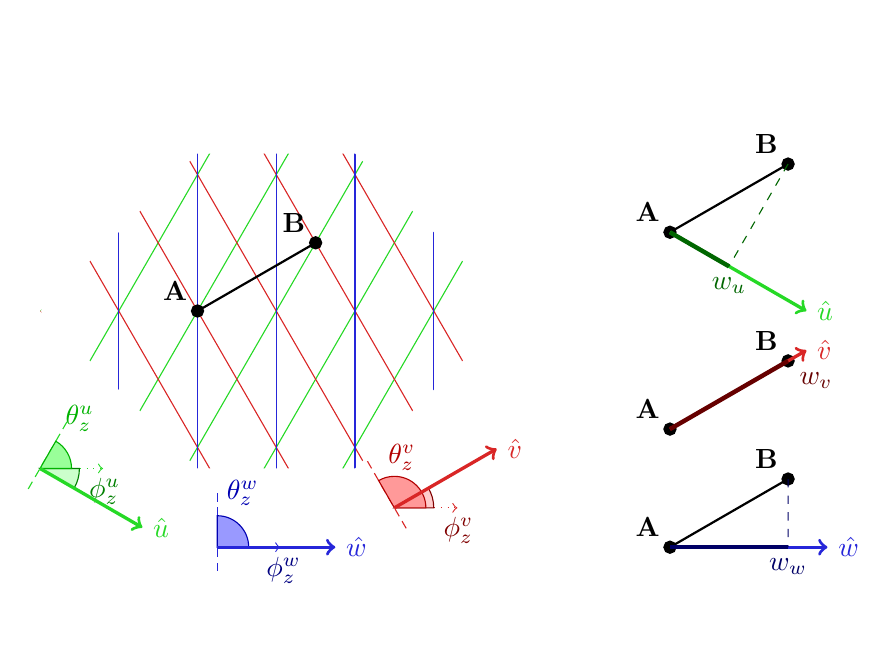
\begin{tikzpicture}
				%
				% a lot of things could be done better in this code
				%
				
				% reference
			%	\draw[step=1,gray!50!white] (-4,-4) grid (4,4);
			%	\fill ( 0, 0 ) circle [radius=2pt];
				
				\def\uName{\ensuremath{u}} \def\uColor{green}
				\def\vName{\ensuremath{v}} \def\vColor{red}
				\def\wName{\ensuremath{w}} \def\wColor{blue}
				
				%  - all wires
				\begin{scope}
					% clipping path
					\path [clip] (-3, +0) -- (-1, +2) -- (+1, +2) -- (+3, 0) -- (+1, -2) -- (-1, -2) -- cycle;
					
					% u plane (\theta_z = \pi/3)
					\draw[gray!30!\uColor] ( -5.0000, -3.4642 ) -- ( -1.0000, +3.4642 );
					\draw[gray!30!\uColor] ( -4.0000, -3.4642 ) -- ( +0.0000, +3.4642 );
					\draw[gray!30!\uColor] ( -3.0000, -3.4642 ) -- ( +1.0000, +3.4642 );
					\draw[gray!30!\uColor] ( -2.0000, -3.4642 ) -- ( +2.0000, +3.4642 );
					\draw[gray!30!\uColor] ( -1.0000, -3.4642 ) -- ( +3.0000, +3.4642 );
					\draw[gray!30!\uColor] ( +0.0000, -3.4642 ) -- ( +4.0000, +3.4642 );
					
					% v plane (\theta_z = 2\pi/3)
					\draw[gray!30!\vColor] ( -5.0000, +3.4642 ) -- ( -1.0000, -3.4642 );
					\draw[gray!30!\vColor] ( -4.0000, +3.4642 ) -- ( +0.0000, -3.4642 );
					\draw[gray!30!\vColor] ( -3.0000, +3.4642 ) -- ( +1.0000, -3.4642 );
					\draw[gray!30!\vColor] ( -2.0000, +3.4642 ) -- ( +2.0000, -3.4642 );
					\draw[gray!30!\vColor] ( -1.0000, +3.4642 ) -- ( +3.0000, -3.4642 );
					\draw[gray!30!\vColor] ( +0.0000, +3.4642 ) -- ( +4.0000, -3.4642 );
					
					% w plane (\theta_z = \pi/2)
					\draw[gray!30!\wColor] ( -2.0000, +3.4642 ) -- ( -2.0000, -3.4642 );
					\draw[gray!30!\wColor] ( -1.0000, +3.4642 ) -- ( -1.0000, -3.4642 );
					\draw[gray!30!\wColor] ( +0.0000, +3.4642 ) -- ( +0.0000, -3.4642 );
					\draw[gray!30!\wColor] ( +1.0000, +3.4642 ) -- ( +1.0000, -3.4642 );
					\draw[gray!30!\wColor] ( +2.0000, +3.4642 ) -- ( +2.0000, -3.4642 );
					
				\end{scope}
				
				% the good part is: just change B relative to A, and the complete
				% plot updates correctly (may need to fix a bit label anchors)
				\def\AtoB{1.5000, +0.8660}
			%	\def\AtoB{+2.0, +0.0}
			%	\def\AtoB{1.5000, -0.8660}
				
				% - points
				\draw [black,thick,->,fill=black] ( -1.0000, +0.0000 ) circle [radius=2pt] node[anchor=south east] {\textbf{A}}
					-- ++(\AtoB) circle [radius=2pt] node[anchor=south east] {\textbf{B}};
				
				% creates a coordinate system description forthe specified wire plane
				% Usage: \axisSystem{plane label}{theta_z}{base color}{vertex placement}
				\newcommand{\axisSystem}[4]{
					\begin{scope}
						\def\axisName{#1}
						\def\axisAngle{#2}
						\def\axisColor{#3}
						\coordinate (vertex) at ( #4 );
						% - axes
						\draw[gray!30!\axisColor,thin,dotted,->] (vertex) -- ++( +0.8000, +0.0000 ); % small z axis
						\draw[gray!30!\axisColor,thin,densely dashed] (vertex) ++(\axisAngle:-0.3) -- ++(\axisAngle:1); % small wire axis
						
						\filldraw[fill=\axisColor!20,draw=\axisColor!50!black]
							(vertex)
							-- ++(0:0.5)
								node[color=\axisColor!50!black,anchor=north west] { $\phi_{z}^{\axisName}$ }
							arc [start angle=0, delta angle=\axisAngle-90, radius=0.5]
							-- cycle ;
						\filldraw[fill=\axisColor!40,draw=\axisColor!70!black]
							(vertex)
							-- ++(0:0.4)
							arc [start angle=0, delta angle=\axisAngle, radius=0.4]
								node[color=\axisColor!70!black,anchor=south west] { $\theta_{z}^{\axisName}$ }
							-- cycle;
						\draw[gray!30!\axisColor,very thick,->] (vertex) -- ++(\axisAngle-90:1.5) node[anchor=west] {$\hat{\axisName}$};
					\end{scope}
				} % axisSystem
				
				\axisSystem{\uName}{ +60}{\uColor}{-3.0000, -2.0000}
				\axisSystem{\vName}{+120}{\vColor}{+1.5000, -2.5000}
				\axisSystem{\wName}{ +90}{\wColor}{-0.7500, -3.0000}
				
				
				% small inset for u plane projection
				\begin{scope}
					\coordinate (vertex) at ( +5.0000, +1.0000 );
					\def\axisName{\uName}
					\def\axisAngle{-30}
					\def\axisColor{\uColor}
					% - points
					\draw [black,thick,->,fill=black] (vertex) coordinate (A) circle [radius=2pt] node[anchor=south east] {\textbf{A}}
						-- ++(\AtoB) coordinate (B) circle [radius=2pt] node[anchor=south east] {\textbf{B}};
					% - axis
					\draw [gray!30!\axisColor,very thick,->,name path=local axis] (A) -- ++(\axisAngle:2) node[anchor=west] {$\hat{\axisName}$};
					\path [name path=projection line] (B) ++(\axisAngle-90:-2) -- ++(\axisAngle-90:4); % go both directions to fin intersection
					\draw [name intersections={of=local axis and projection line, by=w},ultra thick,\axisColor!40!black] (A) -- (w) node[anchor=north] {$w_{\axisName}$};
					\draw [thin,dashed,\axisColor!40!black] (B) -- (w);
				\end{scope}
				
				
				% small inset for v plane projection
				\begin{scope}
					\coordinate (vertex) at ( +5.0000, -1.5000 );
					\def\axisName{\vName}
					\def\axisAngle{+30}
					\def\axisColor{\vColor}
					% - points
					\draw [black,thick,->,fill=black] (vertex) coordinate (A) circle [radius=2pt] node[anchor=south east] {\textbf{A}}
						-- ++(\AtoB) coordinate (B) circle [radius=2pt] node[anchor=south east] {\textbf{B}};
					% - axis
					\draw [gray!30!\vColor,very thick,->,name path=local axis] (A) -- ++(\axisAngle:2) node[anchor=west] {$\hat{\axisName}$};
					\path [name path=projection line] (B) ++(\axisAngle-90:-2) -- ++(\axisAngle-90:4); % go both directions to fin intersection
					\draw [name intersections={of=local axis and projection line, by=w},ultra thick,\vColor!40!black] (A) -- (w) node[anchor=north west] {$w_{\axisName}$};
					\draw [thin,dashed,\vColor!40!black] (B) -- (w);
				\end{scope}
				
				% small inset for w plane projection
				\begin{scope}
					\coordinate (vertex) at ( +5.0000, -3.0000 );
					\def\axisName{\wName}
					\def\axisAngle{+0}
					\def\axisColor{\wColor}
					% - points
					\draw [black,thick,->,fill=black] (vertex) coordinate (A) circle [radius=2pt] node[anchor=south east] {\textbf{A}}
						-- ++(\AtoB) coordinate (B) circle [radius=2pt] node[anchor=south east] {\textbf{B}};
					% - axis
					\draw [gray!30!\wColor,very thick,->,name path=local axis] (A) -- ++(\axisAngle:2) node[anchor=west] {$\hat{\axisName}$};
					\path [name path=projection line] (B) ++(\axisAngle-90:-2) -- ++(\axisAngle-90:4); % go both directions to fin intersection
					\draw [name intersections={of=local axis and projection line, by=w},ultra thick,\wColor!40!black] (A) -- (w) node[anchor=north] {$w_{\axisName}$};
					\draw [thin,dashed,\wColor!40!black] (B) -- (w);
				\end{scope}
				
				
			\end{tikzpicture}
		\end{center}
		\vspace{-4ex} % "center" environment leaves a lot of space afterwards...
		\caption{
			\label{fig:Projections}
			Projection of a segment $AB$ on different wire plane coordinates \emph{(note the different wire pitch)}.
		}
	\end{figure}

	Other definitions:
	\begin{description}
		\item[$\vec{A} = \brackets{ z_{A}, y_{A}, x_{A}}$] absolute coordinate of the starting point $A$ in the TPC volume.
		\item[$\vec{B} = \brackets{ z_{B}, y_{B}, t_{B} }$] absolute coordinate of the ending point $B$ in the TPC volume.
		\item[$\vec{A}^{\prime} = \brackets{ y^{\prime}_{A}, z^{\prime}_{A} }$] projection of point $A$ on any wire plane.
		\item[$\vec{B}^{\prime} = \brackets{ y^{\prime}_{B}, z^{\prime}_{B} }$] projection of point $B$ on any wire plane.
		\item[$\vec{\Delta} \defined \vec{B} - \vec{A}$] vector connecting $A$ to $B$.
		\item[$\vec{\Delta}^{\prime} \defined \vec{B}^{\prime} - \vec{A}^{\prime} = \brackets{ \Delta y, \Delta z }$] projection of $\vec{\Delta}$ on any wire plane, with $\Delta y = y_{B} - y_{A}$ and similarly for $\Delta z$.
		\item[$\thetaDeltaP$] angle of $\vec{\Delta}^{\prime}$ respect to $z$.
		\item[$\Delta t \defined t^{B} - t^{A}$] difference in time coordinate between $A$ and $B$
		\item[$k$] will denote a wire plane (\eg, $u$, $v$...).
		\item[$\theta_{z}^{k}$] angle of the wires on plane $k$ on a given plane respect to $z$ direction.
		\item[$\hat{k} \defined \brackets{\cos \phi^{k}_{z}, \sin \phi^{k}_{z}}$] direction of increasing wire number, perpendicular to the wires of plane $k$. The definition of the origin is irrelevant since we deal only with $w$ differences. Angles $\phi_{z}$ are defined respect to the $z$ axis.
		\item[$p_{k}$] pitch of the wires on plane $k$.
		\item[$\hat{k}^{*} \defined \hat{k} / p_{k}$] the wire coordinate versor, parallel to $\hat{k}$ but translating the global metrics into number of wires.
		\item[$t_{k}$] $t$ coordinate of all the points lying on plane $k$.
		\item[$w^{A}_{k}$, $w^{B}_{k}$] projections of $A^{\prime}$ and $B^{\prime}$ on the direction $\hat{k}^{*}$, in wire unit.
		\item[$\Delta w_{k}$, $\Delta t_{k}$] differences between the observed coordinates of $A$ and $B$ on plane $k$: $\Delta w_{k} \defined w^{B}_{k} - w^{A}_{k}$, $\Delta t_{k} \defined t^{B}_{k} - t^{A}_{k}$
		\item[$s_{k}$] slope observed on plane $k$ from $A^{\prime}$ to $B^{\prime}$: $s_{k} \defined \frac{t^{B}_{k} - t^{A}_{k}}{w^{B}_{k} - w^{A}_{k}} = \frac{\Delta t_{k}}{\Delta w_{k}}$.
		
	\end{description}
	
	
	\section{Goal}
	\label{sec:Goal}
	
	Let some charge be deposited in point $A$ and then point $B$ in the TPC volume.\\
	The deposited charge will drift to the wire planes and hit each of them in projected points $A^{\prime}$ and $B^{\prime}$.\\
	From each wire plane, the projection will be observed as two wire coordinates on their respective time, $\brackets{w^{A}_{k}, t^{A}_{k}}$ and $\brackets{w^{B}_{k}, t^{B}_{k}}$.
	We therefore obtain from each plane a slope $s_{k}$ from $A^{\prime}$ to $B^{\prime}$.\\
	We observe these points for two wire planes $u$ and $v$, and their respective slopes $s_{u}$ and $s_{v}$.\\
	The goal is to compute the value $s_{w}$ of the slope observed on a third plane, as function of $s_{u}$ and $s_{v}$, plus the wire angles $\theta^{u}_{z}$, $\theta^{v}_{z}$ and $\theta^{w}_{z}$.
	
	
	\section{Derivation}
	\label{sec:Derivation}
	
	We first note that the $\Delta t_{k}$ for $k \in \braces{ u, v, w}$ have all the same value even if the single coordinates on each plane are shifted by their respective $t_{k}$.
	Therefore we define the common value $\Delta t \defined \Delta t_{k}$ and the slopes have form $s_{k} = \frac{\Delta t}{\Delta w_{k}}$.
	This sharing of $\Delta t$ also implies
	\begin{equation}
		\label{eq:DeltaT}
		\Delta t = s_{k} \Delta w_{k} = s_{u} \Delta w_{u} = s_{v} \Delta w_{v} = s_{w} \Delta w_{w}
	\end{equation}
	where we'll see that the last three equation members count for two equations with two unknowns: $s_{w}$ and the angle $\thetaDeltaP$ hidden in the $\Delta w$ terms.
	
	In fact, the difference $\Delta w_{k}$ is the projection of $\vec{\Delta}^{\prime}$ on the direction of the wire coordinate of plane $k$:
	\begin{align*}
		\Delta w_{k} &= \vec{\Delta}^{\prime} \cdot \hat{k^{*}} = \Delta y \sin \phi_{z}^{k} / p_{k} + \Delta z \cos \phi_{z}^{k} / p_{k} \nonumber \\
	%	\label{eq:DeltaW}
		             &= \frac{\abs{\vec{\Delta}^{\prime}}}{p_{k}} \brackets{\cos \thetaDeltaP \cos \phi_{z}^{k} + \sin \thetaDeltaP \sin \phi_{z}^{k}}
	\end{align*}
	Let's forget about $\Delta t$ and remove \abs{\vec{\Delta}^{\prime}} from \cref{eq:DeltaT} to get:
	\begin{align}
		\frac{s_{u}}{p_{u}} \brackets{\cos \thetaDeltaP \cos \phi_{z}^{u} + \sin \thetaDeltaP \sin \phi_{z}^{u}} 
		  &= \frac{s_{v}}{p_{v}} \brackets{\cos \thetaDeltaP \cos \phi_{z}^{v} + \sin \thetaDeltaP \sin \phi_{z}^{v}} \nonumber \\
		  &= \frac{s_{w}}{p_{w}} \brackets{\cos \thetaDeltaP \cos \phi_{z}^{w} + \sin \thetaDeltaP \sin \phi_{z}^{w}}
		\label{eq:T}
	\end{align}
	To simplify the notation, we define $s^{*}_{k} = \frac{s_{k}}{p_{k}}$, that represent the slope in space units rather than wire units\footnote{
		We are omitting that $t$ is also not in space units, but rather is number of ticks.
		It is not relevant in this demonstration, because we never work in the real 3D space: we measure $t$ coordinates directly in the first place, and we never need to relate them directly to the $y$ and $z$ coordinates --- we rather compare with wire coordinates.
	}.
	Then, arbitrary picking the last two members and electing $v$ as our ``pilot'' plane, we get a solution for $s^{*}_{w}$:
	\begin{equation}
		\label{eq:sw_general}
		s^{*}_{w} = s^{*}_{v} \frac{\cos \thetaDeltaP \cos \phi_{z}^{v} + \sin \thetaDeltaP \sin \phi_{z}^{v}}{\cos \thetaDeltaP \sin \cos_{z}^{w} + \sin \thetaDeltaP \sin \phi_{z}^{w}}
	\end{equation}
	
	Harvesting a $\cos \thetaDeltaP$ from \cref{eq:T}:
	\begin{align}
		\label{eq:Slopes}
		s^{*}_{u} \brackets{\cos \phi_{z}^{u} + \tan \thetaDeltaP \sin \phi_{z}^{u}} 
		  &= s^{*}_{v} \brackets{\cos \phi_{z}^{v} + \tan \thetaDeltaP \sin \phi_{z}^{v}} \nonumber \\
		  &= s^{*}_{w} \brackets{\cos \phi_{z}^{w} + \tan \thetaDeltaP \sin \phi_{z}^{w}}
	\end{align}
	and, using the first two members:
	\begin{equation*}
		\label{eq:tanAB}
		 \tan \thetaDeltaP = - \frac{s^{*}_{u} \cos \phi_{z}^{u} - s^{*}_{v} \cos \phi_{z}^{v}}{s^{*}_{u} \sin \phi_{z}^{u} - s^{*}_{v} \sin \phi_{z}^{v}}
	\end{equation*}
	If $\cos \thetaDeltaP \ne 0$, $\tan \thetaDeltaP$ is finite and we can replace its expression into \cref{eq:Slopes} to get:
	\begin{align}
		\label{eq:sw_assumption}
		s^{*}_{w} &= s^{*}_{v} \frac{\cos \phi_{z}^{v} + \tan \thetaDeltaP \sin \phi_{z}^{v}}{\cos \phi_{z}^{w} + \tan \thetaDeltaP \sin \phi_{z}^{w}} \nonumber \\
		      &= s^{*}_{v} \frac{\brackets{s^{*}_{u} \sin \phi_{z}^{u} - s^{*}_{v} \sin \phi_{z}^{v}}\cos \phi_{z}^{v} - \brackets{s^{*}_{u} \cos \phi_{z}^{u} - s^{*}_{v} \cos \phi_{z}^{v}} \sin \phi_{z}^{v}}{\brackets{s^{*}_{u} \sin \phi_{z}^{u} - s^{*}_{v} \sin \phi_{z}^{v}}\cos \phi_{z}^{w} - \brackets{s^{*}_{u} \cos \phi_{z}^{u} - s^{*}_{v} \cos \phi_{z}^{v}} \sin \phi_{z}^{w}} \nonumber \\
		      &= s^{*}_{v} \frac{s^{*}_{u} \brackets{\sin \phi_{z}^{u} \cos \phi_{z}^{v} - \cos \phi_{z}^{u} \sin \phi_{z}^{v}}}
		      {s^{*}_{u} \brackets{\sin \phi_{z}^{u} \cos \phi_{z}^{w} - \cos \phi_{z}^{u} \sin \phi_{z}^{w}} - s^{*}_{v} \brackets{\sin \phi_{z}^{v} \cos \phi_{z}^{w} - \cos \phi_{z}^{v} \sin \phi_{z}^{w}} } \nonumber \\
		      &= \frac{s^{*}_{u} s^{*}_{v} \sin \brackets{\phi_{z}^{u} - \phi_{z}^{v}}}
		      {s^{*}_{u} \sin \brackets{\phi_{z}^{u} - \phi_{z}^{w}} - s^{*}_{v} \sin \brackets{\phi_{z}^{v} - \phi_{z}^{w}}} \nonumber \\
		      &= \frac{\sin \brackets{\phi_{z}^{u} - \phi_{z}^{v}}}
		      {\frac{1}{s^{*}_{v}} \sin \brackets{\phi_{z}^{u} - \phi_{z}^{w}} - \frac{1}{s^{*}_{u}} \sin \brackets{\phi_{z}^{v} - \phi_{z}^{w}}}
	\end{align}
	Note that in the second line the singularity for $\cos \thetaDeltaP = 0$ disappears; in that case, $s^{*}_{w} = s^{*}_{v} \frac{\sin \phi_{z}^{v}}{\sin \phi_{z}^{w}}$, consistently with \cref{eq:sw_general}.
	
	This result is expressed in terms of the $\phi^{k}_{z}$ angles.
	A subtle and yet critical point is to understand the definition of $\theta^{k}_{z}$:
	the axis of a wire can be defined by an angle $\theta^{k}_{z}$ as well as by $\ppi + \theta^{k}_{z}$.
	This turns into two possible definitions:
	$\phi_{z}^{k} = \theta^{k}_{z} - \pi/2$
		($\hat{k}$ and the wire direction $\hat{w}_{k}$ define a positive base: $\hat{k} \times \hat{w}_{k} = +1$)
	and $\phi_{z}^{k} = \theta^{k}_{z} + \pi/2$
		($\hat{k} \times \hat{w}_{k} = -1$).
	Let's consider case by case the effect on \cref{eq:sw_assumption}:
	\begin{description}
		\item[all angles consistently defined], $\phi_{z}^{k} = \theta^{k}_{z} \pm \pi/2$ with the same sign for all $k$: $\phi_{z}^{k_{1}} - \phi_{z}^{k_{2}} = \theta_{z}^{k_{1}} - \theta_{z}^{k_{2}}$, yielding to the same expression:
			\begin{equation*}
				\frac{\sin \brackets{\theta_{z}^{u} - \theta_{z}^{v}}}
					{\frac{1}{s^{*}_{v}} \sin \brackets{\theta_{z}^{u} - \theta_{z}^{w}} - \frac{1}{s^{*}_{u}} \sin \brackets{\theta_{z}^{v} - \theta_{z}^{w}}}
			\end{equation*}
		\item[target angle defined differently than the others], $\phi_{z}^{u,v} = \theta_{z}^{u,v} \pm \pi/2$ (with the same sign) and $\phi_{z}^{w} = \theta_{z}^{w} \mp \pi/2$: the numerator is unchanged, while since $\phi_{z}^{u,v} - \phi_{z}^{w} = \theta_{z}^{u,v} - \theta_{z}^{w} \pm \pi$, the denominator flips sign:
			\begin{equation*}
				\frac{\sin \brackets{\theta_{z}^{u} - \theta_{z}^{v}}}
					{- \frac{1}{s^{*}_{v}} \sin \brackets{\theta_{z}^{u} - \theta_{z}^{w}} + \frac{1}{s^{*}_{u}} \sin \brackets{\theta_{z}^{v} - \theta_{z}^{w}}}
			\end{equation*}
		\item[pilot angle defined differently], $\phi_{z}^{u,w} = \theta_{z}^{u,w} \pm \pi/2$ (with the same sign) and $\phi_{z}^{v} = \theta_{z}^{v} \mp \pi/2$: only the sign of the term with $\phi_{z}^{u} - \phi_{z}^{w}$ does not change sign:
			\begin{equation*}
				\frac{ - \sin \brackets{\theta_{z}^{u} - \theta_{z}^{v}}}
					{\frac{1}{s^{*}_{v}} \sin \brackets{\theta_{z}^{u} - \theta_{z}^{w}} + \frac{1}{s^{*}_{u}} \sin \brackets{\theta_{z}^{v} - \theta_{z}^{w}}}
			\end{equation*}
		\item[non-pilot input angle defined differently], $\phi_{z}^{v,w} = \theta_{z}^{v,w} \pm \pi/2$ (with the same sign) and $\phi_{z}^{u} = \theta_{z}^{u} \mp \pi/2$: only the sign of the term with $\phi_{z}^{v} - \phi_{z}^{w}$ does not change sign:
			\begin{equation*}
				\frac{\sin \brackets{\theta_{z}^{u} - \theta_{z}^{v}}}
					{\frac{1}{s^{*}_{v}} \sin \brackets{\theta_{z}^{u} + \theta_{z}^{w}} - \frac{1}{s^{*}_{u}} \sin \brackets{\theta_{z}^{v} - \theta_{z}^{w}}}
			\end{equation*}
	\end{description}
	Given this complication, it's better to think and code in terms of $\phi_{z}^{k}$.
	
	
	\section{Result}
	\label{sec:Result}
	
	Given the definitions above, the slope observed on plane $w$ is expressed as:
	\begin{equation}
		s_{w} = \frac{p_{w} \sin \brackets{\phi_{z}^{u} - \phi_{z}^{v}}}
		      {\frac{p_{v} }{s_{v}} \sin \brackets{\phi_{z}^{u} - \phi_{z}^{w}} - \frac{p_{u}}{s_{u}} \sin \brackets{\phi_{z}^{v} - \phi_{z}^{w}}}
		\label{eq:sw}
	\end{equation}
	The singularity describes the case where the projected segment $\vec{\Delta}^{\prime}$ is perpendicular to the wire we are testing, that is where $\Delta w_{w} = 0$.
	In that case, the slope is effectively infinity.
	
	Expressing $s_{w}$ as function of $\theta_{z}^{k}$ instead of $\phi_{z}^{k}$ yields to such complications,
	that it's easier to compute $\phi_{z}^{k}$ first, and then use \cref{eq:sw}.
	
\end{document}
%%%%%%%%%%%%%%%%%%%%%%%%%%%%%%%%%%%%%%%%%%%%%%%%%%%%%%%%%%%%%%%%%%%%%%%%%%%%%%%%
